\chapter{Concept Testing}

\textit{In this chapter, different components of the proof of concept outlined in \cref{chap:method} will be tested and the results shown. This will be done using a combination of data made available online under an open license and original data collected. First, the components of SHS will be tested individually. Hereafter the whole SHS-PF with activity recognition will be treated.}

\section{Step Detection}
\citet{Salvi2018} have released the data used for their step detection algorithm under an open license. This includes a validation dataset where a ground truth device was used. The ground truth device consisted of sensors placed in the soles of the test subject's shoes. These devices could measure when the foot applied pressure to the sole of the shoe, indicating contact with the floor, hence when a step is taken. This dataset provides the opportunity to assess the performance of different step detection techniques with a ground truth.\par

The raw data of the validation set consists of sampling time and three raw accelerometer axis signals. In addition, it indicates when a new step has been detected by the ground truth device, and steps detected by the researcher's algorithm. The validation sets contain data of two users carrying the phones in different carrying modes. These are in an armband, back pocket, bag, front pocket, hand, and neck pouch. The device is carried in each carrying mode individually.\par

An extract of this data can be found in \cref{fig:gt_steps_vs_salvi_steps}, showing the accelerometer magnitude of each carrying mode for one user. It also contains points indicating the ground truth steps and the steps detected by the \citet{Salvi2018} algorithm. The figure highlights how the carrying mode affects the characteristics of the acceleration trace. For example, between carrying the smartphone in an armband and front pocket, the former has a much more gradual change with a clear sinusoidal form, while the latter has a larger range of accelerations with much more abrupt changes. 


\begin{figure}[H]
	\centering
	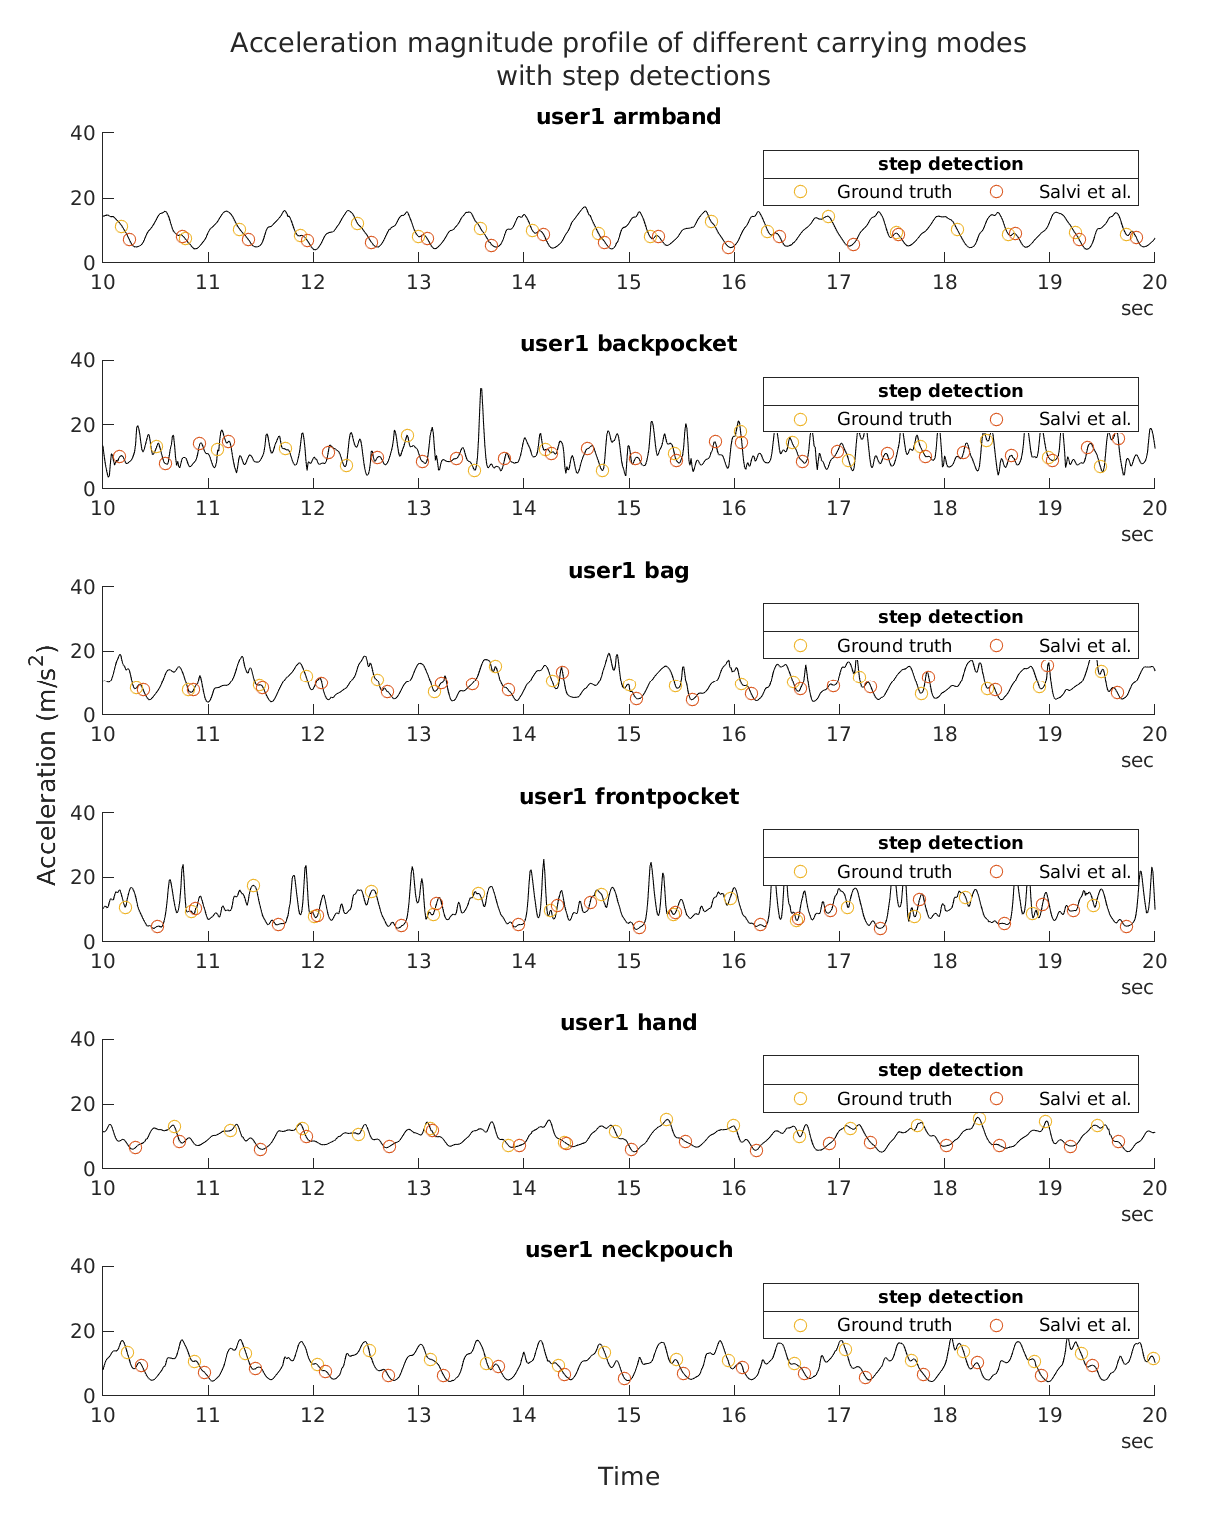
\includegraphics[width=\linewidth]{images/20201112_1318_gt_steps_vs_salvi_steps_1}
	\caption[Step detection validation data]{Extract of validation dataset from \citet{Salvi2018}, indicating ground truth steps and step detected by their algorithm.}
	\label{fig:gt_steps_vs_salvi_steps}
\end{figure}

\newpage
The step detection implementation outlined in Algorithm \ref{algo:step_detect} was applied to the validation data of the researchers, allowing for direct comparison. \cref{fig:sd_abs_comparison} indicates the absolute number of steps detected. \cref{fig:sd_percent_comparison}  shows the percentage error compared to the ground truth, where positive percent error indicates over-counting, while negative undercounting. The results indicate that the implementation performs overall similar to the method of the researchers.  The best performing implementation switches per user and carrying mode, with many carrying modes close to 5\% or less percentage error to the number of steps taken. \par 
From the data, it is also apparent that with the case of "user1 back pocket" that there is a large percentage error for both approaches, something not seen for the same carrying mode with the other user. 
 
	\begin{figure}[htbp]
		\centering
		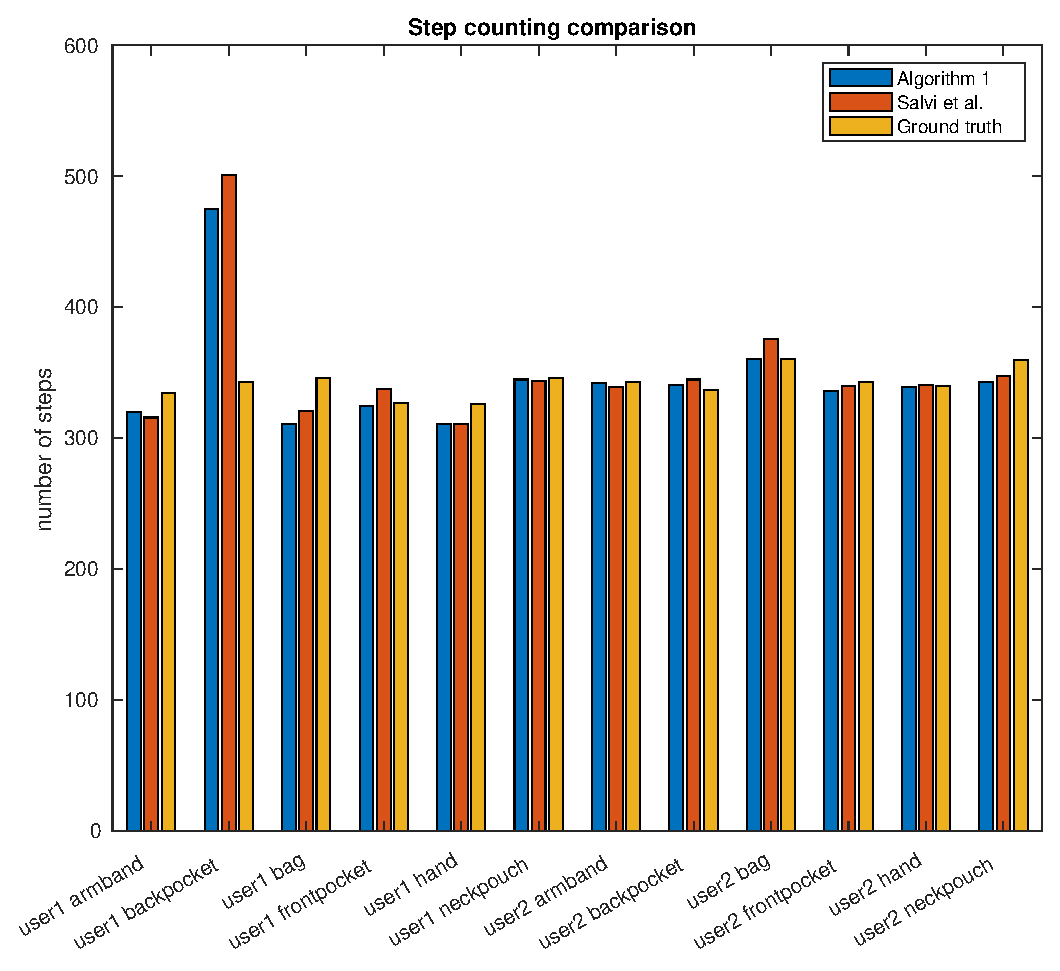
\includegraphics[width=0.7\linewidth]{images/20201112_1347_step_counting_comparison_1}
		\setlength{\belowcaptionskip}{-20pt}
		\caption{Absolute number of steps counted.}
		\label{fig:sd_abs_comparison}
	\end{figure}
\restoregeometry

	\begin{figure}[H]
		\centering
		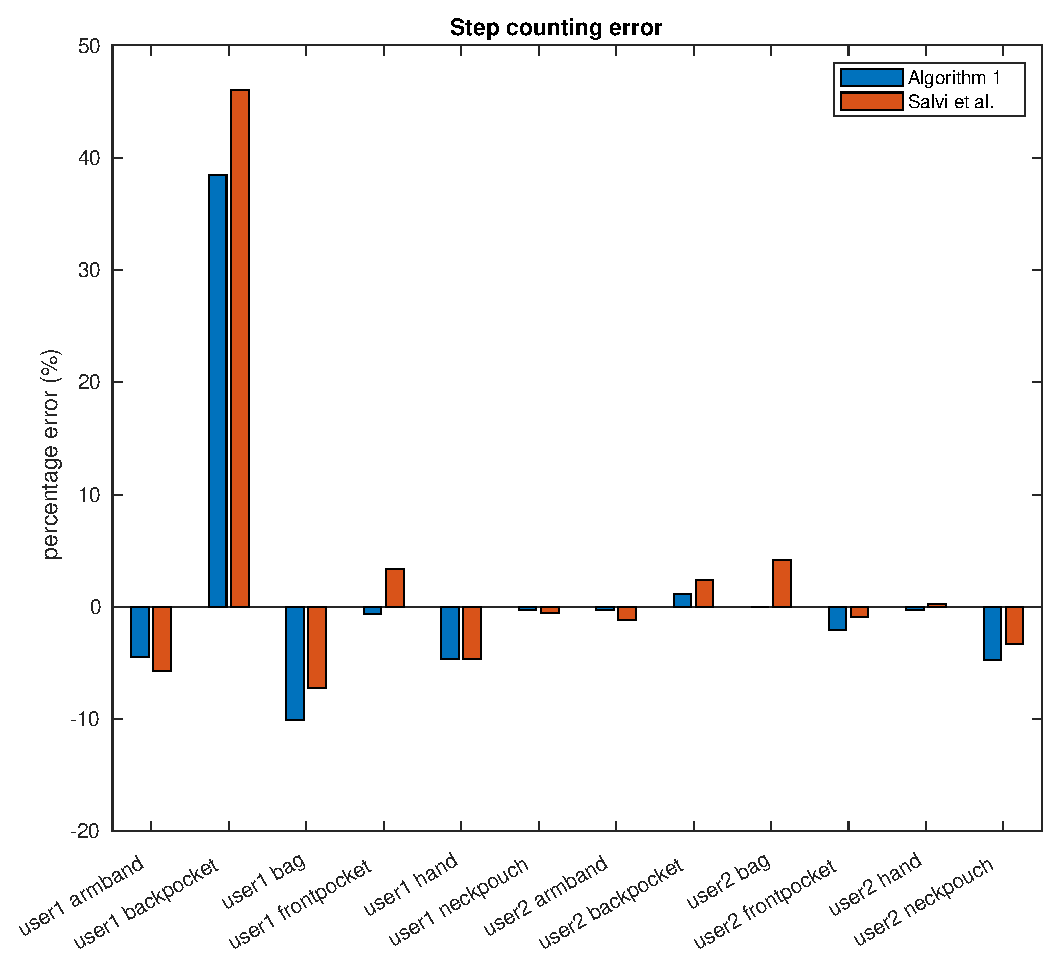
\includegraphics[width=0.7\linewidth]{images/20201112_1401_Step_counting_error}
		\caption{Percentage error from ground truth number of steps. }
		\setlength{\belowcaptionskip}{-2cm}
		\label{fig:sd_percent_comparison}
	\end{figure}
%	\caption[Step detection comparison]{Comparison between \citet{Salvi2018} step detection algorithm, \cref{algo:step_detect} and ground truth for different carrying modes.}
%	\label{fig:sd_comparison}
In addition to the data made available online, original data was gathered outdoors in which a test subject walked exactly 60 steps in a straight line while having a smartphone in 3 different carrying modes, back pocket, front pocket, and in hand. Two trials per carrying mode were performed. The steps were counted manually. The percentage error from the ground truth can be seen in \cref{fig:202009291013step_counting_error_of_60_steps}.
\begin{figure}[H]
	\centering
	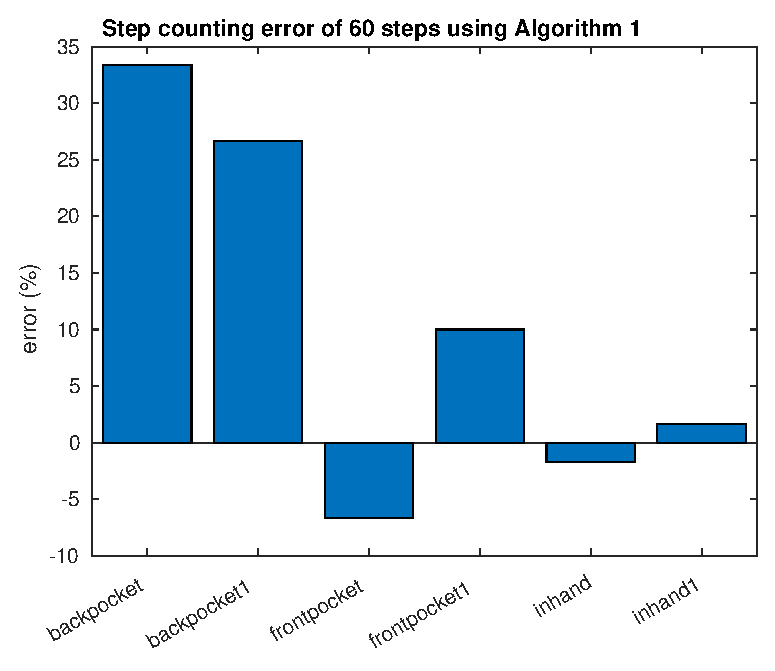
\includegraphics[width=0.6\linewidth]{images/20201112_1406_Step_counting_error_of_60_steps_using_Algorithm_1}
	\setlength{\belowcaptionskip}{-20pt}
	\caption{Original data step counting}
	\label{fig:202009291013step_counting_error_of_60_steps}
\end{figure}

For a \ac{SHS} it is not enough for the number of steps to be accurate, but also the time when a step actually occurs. Detecting a step, combined with the heading orientation at that moment, determines the vector in which the position estimate of the pedestrian will move. It is therefore preferable for a detection to be as close as possible to when a step actually occurs, with no other detections in the vicinity. \par
Using the online data, the time difference between a step detection and its closest ground truth point was calculated per trial. The mean and standard deviation of the time difference was calculated, shown in \cref{fig:202011130914smallest_diff_to_gt_1}.\\ Looking at the results, this metric indicates that the two approaches are similar. The results show that most detections are within 0.1 seconds from the closest ground truth point. The best performing algorithm switches per carrying mode. The \citet{Salvi2018} algorithm detects the step after it has been taken, while \cref{algo:step_detect} slightly before. The large standard deviations for "user2 armband" seems to be caused by both step detection methods having already counted multiple steps before the ground truth device has registered any.

\begin{figure}[H]
	\centering
	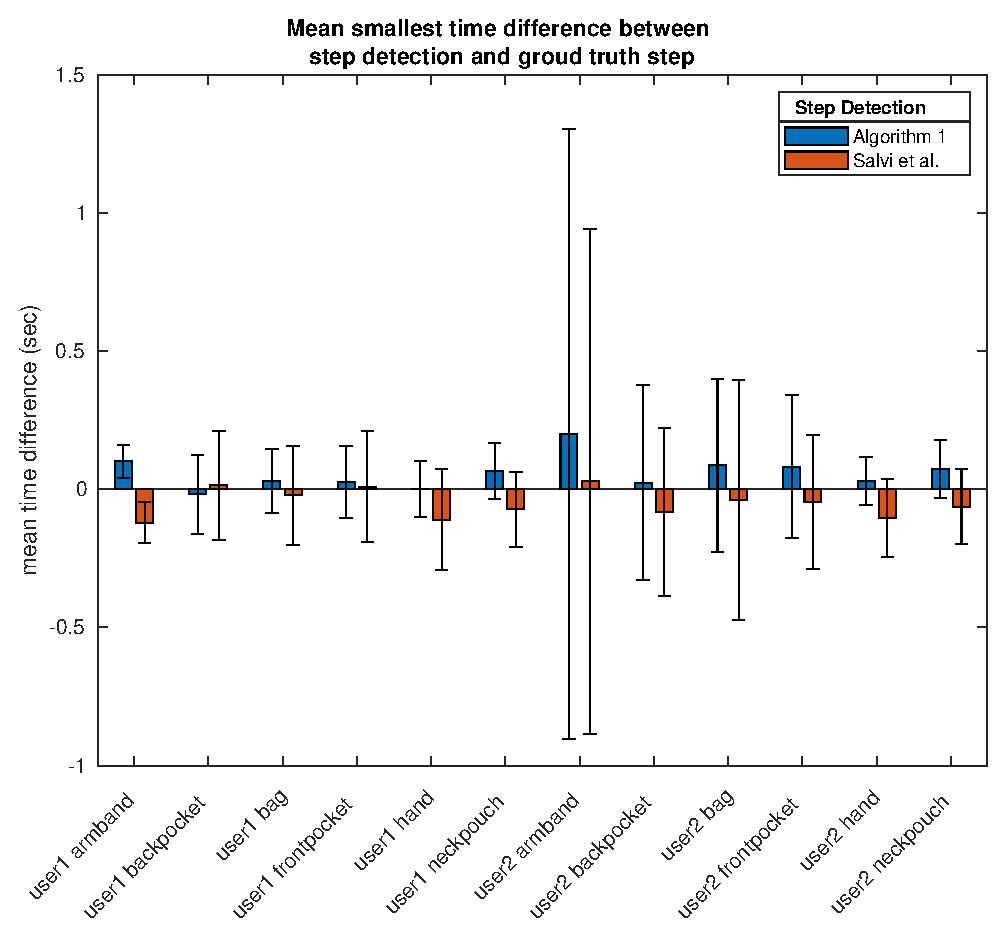
\includegraphics[width=0.7\linewidth]{images/20201113_0914_smallest_diff_to_gt_1}
	\caption{Mean and standard deviation of the smallest time different between step detection and step occurrence. Positive difference indicates detection before step occurrence and negative after occurrence}
	\label{fig:202011130914smallest_diff_to_gt_1}
\end{figure}

One problem with this metric is that two subsequent detections may have the same ground truth point as the nearest point, indicating that there is no unique detection of the step occurring. In order to ascertain how both the \citet{Salvi2018} algorithm and \cref{algo:step_detect} perform in this respect, an approach to "unique" step detection was determined. Since it is unrealistic to expect the step detection to be at the exact time an actual step occurs, intervals are defined where if both an actual step occurs and is detected within the interval, the detection counts as a unique step. An illustrative representation of this can be found in \cref{fig:202011121558_true_positive_example_1}. Here an interval, represented by the green region in the graph is made around one of the ground truth points, visible in the middle of the region and circled in red. If in this interval two steps are detected, no unique step is indicated. In the example of  \cref{fig:202011121558_true_positive_example_1},  \cref{algo:step_detect} would be considered a unique step, while the \citet{Salvi2018} algorithm would not, since there are two detection within the interval.

\begin{figure}
	\centering
	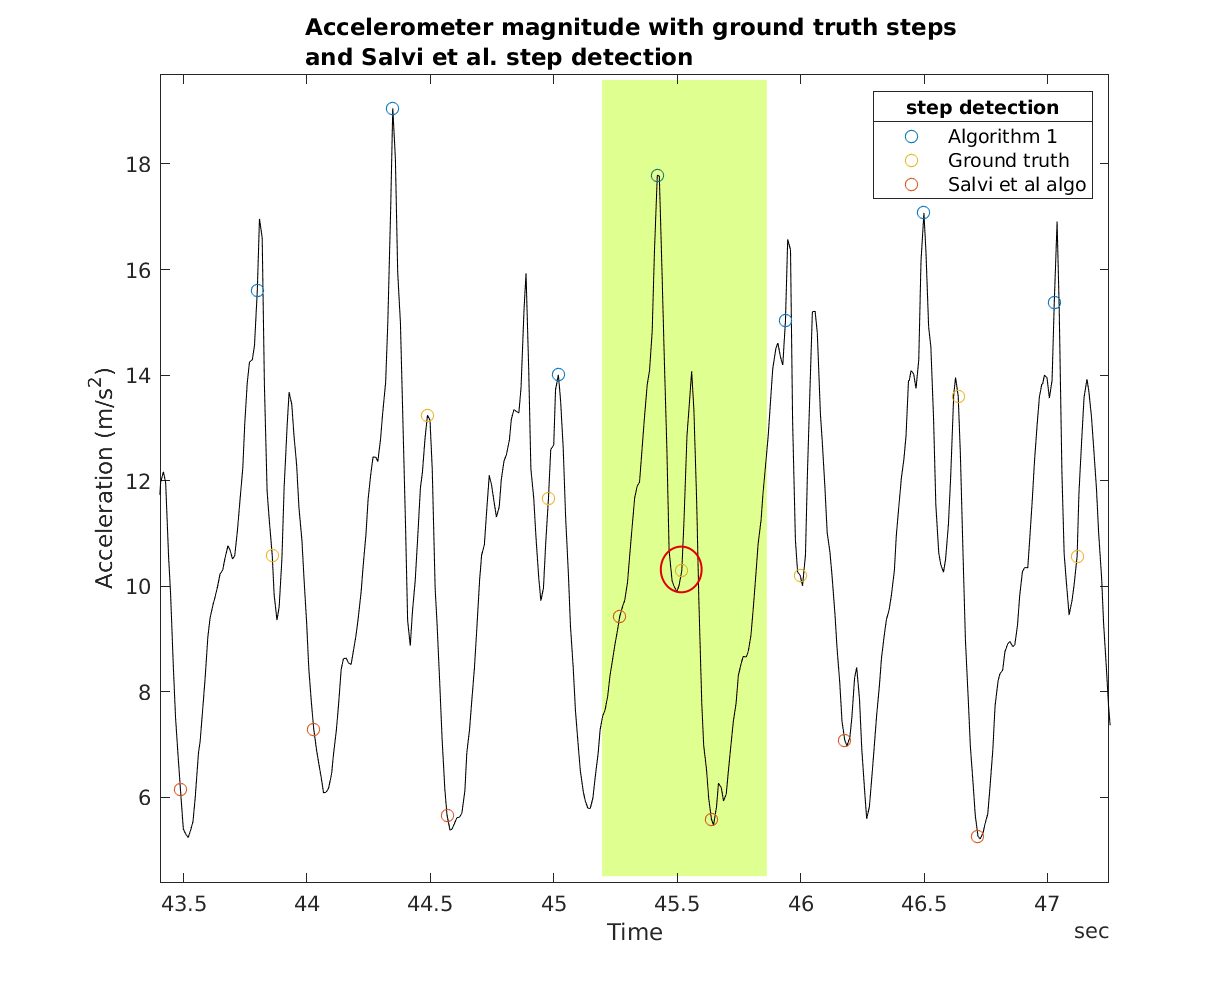
\includegraphics[width=0.75\linewidth]{images/20201112_1809_true_positive_example_2}
	\caption{Representation of interval search method. The light green region represents the search interval around the \citet{Salvi2018} point in the middle.}
	\label{fig:202011121558_true_positive_example_1}
\end{figure}

The time interval is increased iteratively in an attempt to find the highest unique step counts for both algorithms. The results for each user and carrying mode can be found in \cref{fig:sd_tp_fp_comparison}. The results show that while the total number of steps detected are similar between the two approaches, Algorithm \ref{algo:step_detect} has a higher "unique" step detection. This discrepancy between approaches can potentially be explained by the android implementation of the researchers. 

\begin{figure}[H]
	\centering
	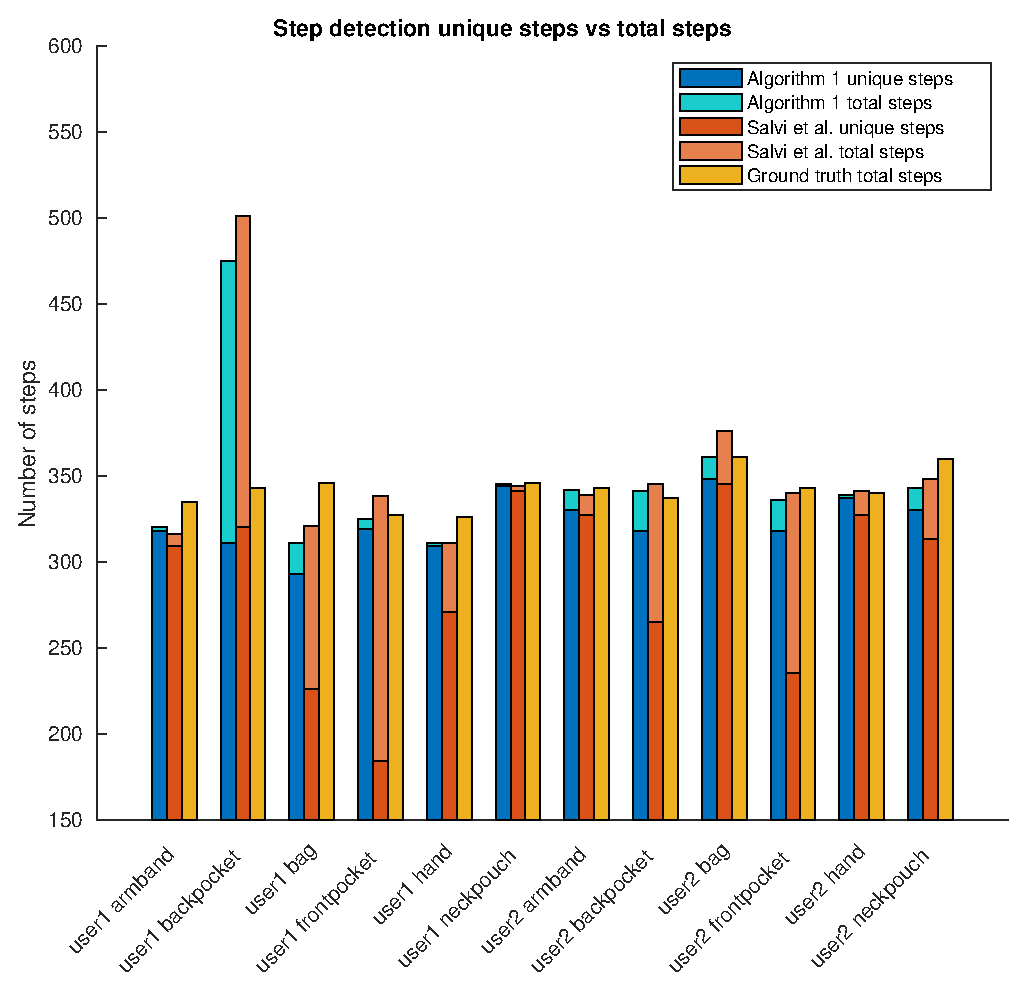
\includegraphics[width=0.7\linewidth]{images/20201112_1857_Step_detection_unique_steps_vs_total_steps_}
	\put(10,10){hello}
	\setlength{\belowcaptionskip}{-20pt}
\caption[False positives and true positives step detection comparison]{Comparison between false positives and true positives for \citet{Salvi2018} step detection and Algorithm \ref{algo:step_detect}}
\label{fig:sd_tp_fp_comparison}
\end{figure}

\section{Step Length Estimation}

\citet{Vezocnik2019} data, available under an open license, consists of smartphone accelerometer data of 15 different people for three walking speeds and in four different carrying modes. Metrics for each test subject are collected, including height, gender, and leg length. The walking speeds were qualitative, in that they were either slow, normal, or fast. The carrying modes include the smartphone in a front pocket, in a bag, in the hand with the phone screen parallel to the floor, and in hand will swinging the carrying arm. Each person has two measurements for each combination of carrying mode and walk speed, one for a 15-meter long straight path and another for a 108-meter long straight path. The smaller set is used to determine parameters for step length estimation methods, while the longer distance is used as a performance measure. This same process will be used to determine the performance of step detection and step length estimation.\\
The best performing algorithm for global parameters is reiterated for convenience,

\begin{equation}
	\label{eq:Tian2016_sle2}
	\text{step size} = K \cdot h \cdot, \sqrt{F}.
\end{equation}


 where $h$ is the user's height and $F$ is the step frequency. It will be referred to as the \citet{Tian2016} approach. The best algorithm for individual parameters is 
 
 \begin{equation}
 	\text{step size} =K \sqrt[4]{A_{\max }-A_{\min }},
 	\label{eq:weinberg_stepsize2}
 \end{equation}
 
 where $A_{max}$ and $A_{min}$ are the maximum and minimum acceleration within a step interval. This will be refered to as the \citet{Weinberg2002} approach. The two approaches will be used and compared to see if similar results are achieved as within \cite{Vezocnik2019}.

In order to determine the tunable parameter $K$ correctly for both approaches, it needs to be used with the output of the step detection algorithm. The step detection algorithm cannot guarantee that all steps are counted, potentially affecting the tunable parameter for both methods. 
The smartphone in hand carrying mode in the data from \cite{Vezocnik2019} will be used for further analysis since step detection indicate it as a carrying mode with low step detection errors. \par

The results for the \citet{Tian2016} approach are shown in \cref{fig:step_length_tian}. Each test subject is shown as a different color with the form of the different markers indicating the speed at which that trial was walked at. The positive linear trend indicated in \cite{Tian2016} can be observed as walking speed increases. In order to find the universal constant $K$, a least square estimation is performed across all data points. The result is shown by the green striped line in the plot. 

	\begin{figure}[H]
	\centering
	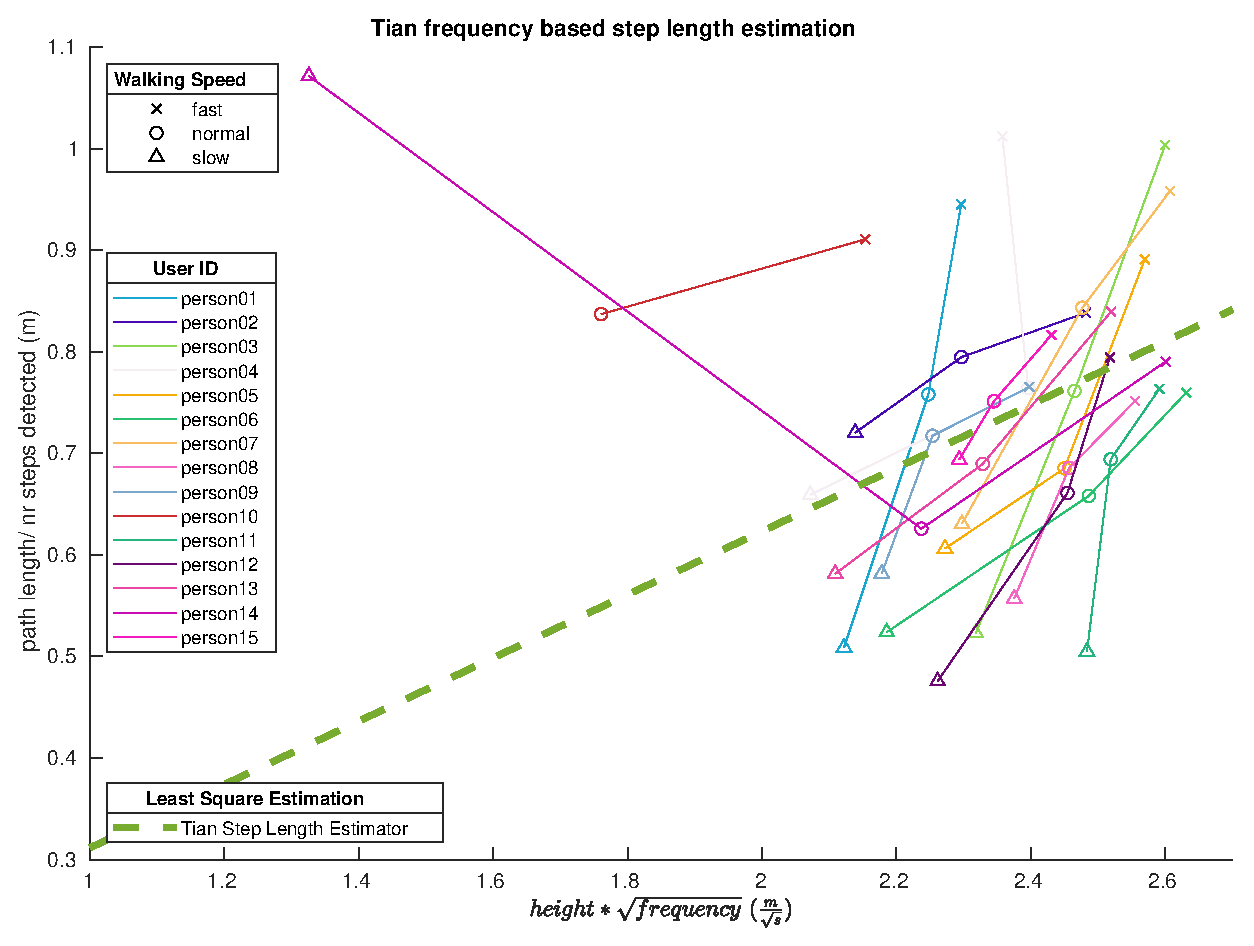
\includegraphics[width=0.8\linewidth]{images/20201113_1634_tian}
	\caption{Opensource step length data with \citet{Tian2016} parameters, indicating linear trend with increasing walking speed.}
	\label{fig:step_length_tian}
	\end{figure}
	
A similar plot is shown in \cref{fig:step_length_weinberg}, but for the \citet{Weinberg2002} approach variables. Here too a positive trend is suggested. Since the \citet{Weinberg2002} works best for personalized variable the tunable parameter is calculated per test subject, instead of all together as with the \citet{Tian2016} approach. 

\begin{figure}[H]
	\centering
	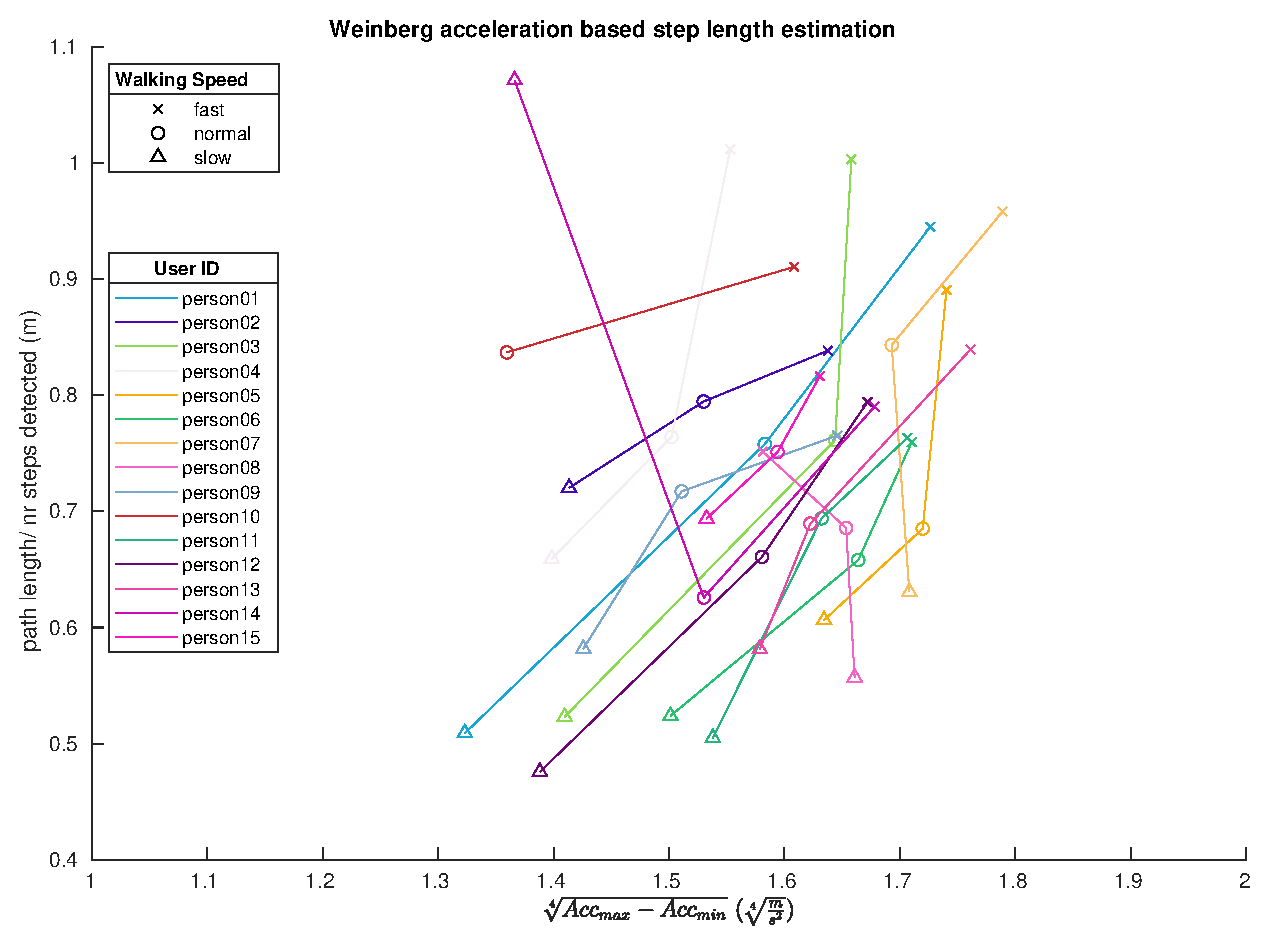
\includegraphics[width=0.8\linewidth]{images/20201113_1639_weinberg}
	\caption{Opensource step length data with \citet{Weinberg2002} parameters, also indicating linear trend with increasing walking speed.}
	\label{fig:step_length_weinberg}
\end{figure}

While most data seems to follow the general linear relationship for both approaches, there are two samples that do not. The two potentially faulty data points are the slow walking sample of both person 10 and 14. For the former, no steps have been detected and are therefore not visible in the plots, while for the latter too few steps have been detected. For person 14, 14 steps have been detected for slow walking, which is fewer steps than when the subject was walking fast. This is either a wrong step detection occurring, or the user walks slowly with very large steps. It is difficult to determine why this is occurring. It could be that during this sample, the test subject was holding the phone incorrectly, the person had a very different step strategy when performing at this speed, or the phone was malfunctioning. This outlier affects the eventual tunable parameter for both step length approaches. Removing it will change the estimate of $K$ from 0.3116 to 0.3080. The validation dataset can be used to determine if the difference in the tunable parameter has a significant effect on the total distance traveled. The difference was found to have a negligible effect on the outcome of the method.
%The results are found in  \cref{fig:step_length_estimation_validation}, where the absolute distance error for all walking speeds for all test subjects are shown, indicated by the dataset ID.
%\begin{figure}[H]
%	\centering
%	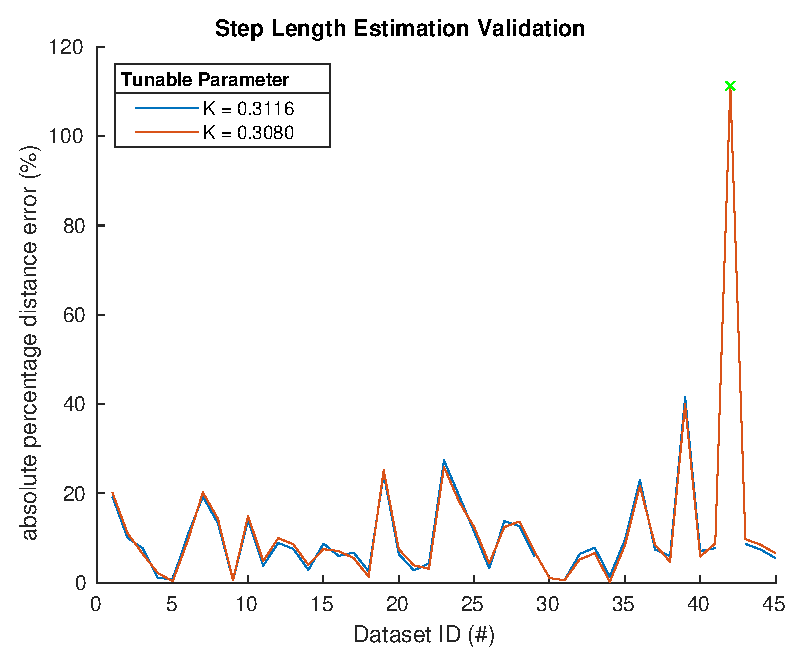
\includegraphics[width=0.65\linewidth]{images/20201028_1344_Step_Length_Estimation_Validation}
%	\setlength{\belowcaptionskip}{-30pt}
%	\caption{Step length estimation using validation dataset}
%	\label{fig:step_length_estimation_validation}
%\end{figure}

The performance of both step length estimators is evaluated by applying them to the data of the longer walking distance and comparing the estimate with the actual distance walked. The results are shown in  \cref{fig:202011131943_wienberg_vs_tian_vezocnik_data1}. This data surprisingly shows that depending on the test subject one or the other method is better at estimating distance traveled at different walking speeds. This does not coincide with the results of \cite{Vezocnik2019}, where personal parameters performed better than general parameters.

What is noticeable from the results is that there is an outlier. This is with the slow walking speed of test subject 14, which is are also the test subject with which the tunable parameter estimation had an outlier. This outlier further supports that there is something significantly different when this test subject is performing at this walking speed.\par 

 Without the outlier, the mean absolute error for \citet{Tian2016} method is 9.7 percent with a standard deviation of 8.0 percent. For the \citet{weinberg} method the mean is 10.38 percent error with a standard deviation of 7.8 percent error. Both results differ from those cited by \cite{Vezocnik2019}, which indicate a mean of 7 percent with a standard deviation of 5 percent for \citet{Tian2016} and 3 percent with a 2.5 percent standard deviation.

\par

\begin{figure}[H]
	\centering
	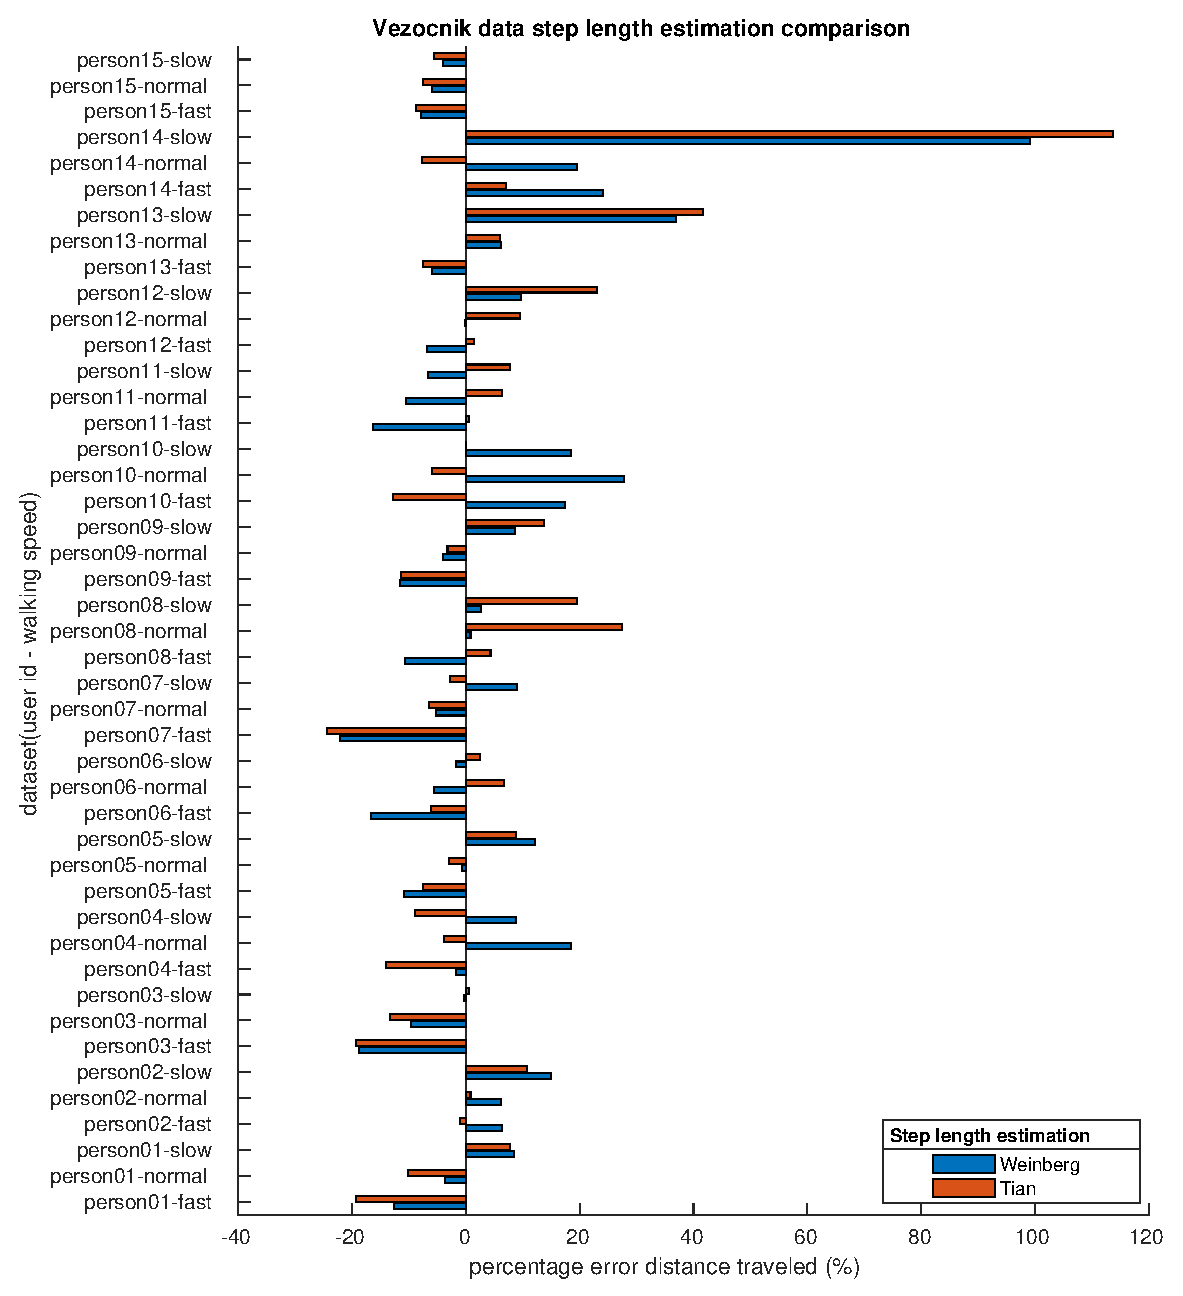
\includegraphics[width=\linewidth]{images/20201113_1943_wienberg_vs_tian_vezocnik_data_1}
	\caption{}
	\label{fig:202011131943_wienberg_vs_tian_vezocnik_data1}
\end{figure}
 
A small scale experiment was performed outdoors using the same process as in \cite{Vezocnik2019}, where a small distance was used for parameter estimation and a longer for performance measurement. Original data was collected from the same person and device used in the eventual indoor localization experiment. Three trials of 30 meters were walked at different qualitative walking speeds, slow, normal, and fast, while recording accelerometer data. Four longer trials of 300 meters were walked, to determine performance, also at different walking speeds. \par 
During the smaller walking distances, the number of steps taken was recorded manually. For two trials the number of steps detected was exactly the number of steps taken. This was for slow and fast walking where 67 and 50 steps were counted respectively.  For the other trial, the detection was off 2 steps, with 57 steps being taken and 55 being recorded. \par 
The different step length estimation methods were applied to the original data. The \citet{Tian2016} method used the same parameter determined for the online dataset. The \citet{Weinberg2002} parameter was based on the smaller distance data. The results are shown in \cref{fig:step_length_personal_testing}. The results seem to suggest that for slow to normal walking the \citet{Tian2016} method works best, with a chance of underestimating the distance traveled For normal to fast walking the \citet{Weinberg2002} method works better, with a chance of overestimating the distance traveled. Making the assumptions that walking indoor is generally more in the normal to slow speed, the choice was made to use the \citet{Tian2016} method for step length estimation in the overall system.
\begin{figure}[H]
	\centering
	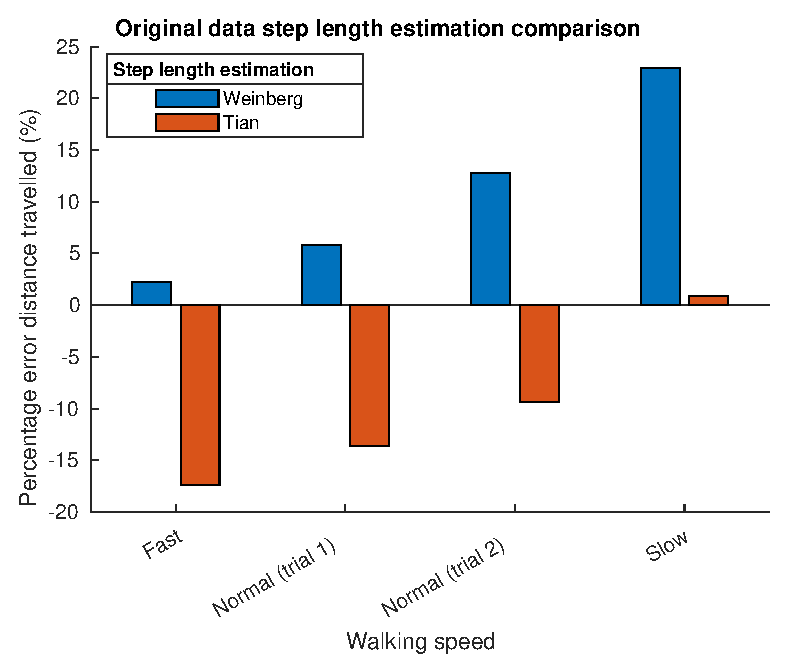
\includegraphics[width=0.7\textwidth]{images/20201113_1920_wienberg_vs_tian_og_data_1}
	\caption{Original data step length estimation \\ }
	\label{fig:step_length_personal_testing}
\end{figure}

\section{Indoor Orientation Estimation}

The step detection and step length estimation experiments were performed outdoors since the location has no effect on accelerometer readings and outdoor testing allows for long walking distances. Orientation estimation and the whole system performance naturally are location-dependent, and will have to be tested indoors. \par

Indoor testing was located at the house of a family member. The test consisted of walking around indoors with a smartphone in hand, and recording the IMU signals in the phone through a dedicated android app. Using the smartphone data, the SHS trajectory could be calculated. During the experiment, a total of 6 successful trials were walked by one test subject, each trying to generate a different trajectory than the previous trials. This same test subject was also used for step detection and step length estimation experiments.

\section{Overall System Testing}

During the experiment, a smartwatch was worn around the wrist of the hand that was not holding the smartphone. This hand was used to open and close doors. The opening of doors was also recorded through the app on the smartphone, which had a button to record timestamps when pressed. The full experimental process can be found in \cref{appendix:shs_experiment}. \par

The smartwatch accelerometer data was synchronized with the smartphone data. The activity recognition method in \cref{sec:method-AR} was used to try and detect door interaction. Combining the activity detection and  with the floor map generated in \cref{sec:method-pf}, the whole system could be tested. For initialization a known starting location on the map was indicated, around which the particles were distributed with a Bayesian profile.  \par 

In addition to recording IMU data from both smartphone and watch while the path was being walked, the trials were also being filmed from a breast pocket by another smartphone. The video recorded during the experiment was used to get a rough estimate of the path walked during the trial. This was done by replaying the video and pausing it at one second intervals. At the paused moments, the test subject position was manually indicating on the map The position and time elapsed since the start of the trial were recorded. The resulting trajectory can be used to give some performance indication of the devised method. \par 

\subsection{With "perfect" activity recognition}
During the experiment the possibility existed of recording a timestamp to indicate the beginning of interaction with a door within the indoor environment. This could be used as a ground truth comparison for eventual activity recognition, but also as a way of representing perfect activity recognition. The recorded timestamps can be used as a particle filter measurement update. Using this method the potential affect of activity recognition for indoor localization can be evaluated, by comparing performance when this form of measurement is used and not used. \par 

All trials were run through the complete system with the manually recorded door interactions, with 3000 particles. This was done for five iterations per trial, in order to show reproducibility.  The resulting estimated trajectory was then compared with the rough estimate generated from video.  A root mean square error was calculated between the two, the results of which can be found in \cref{fig:pf_boxplot}.

\begin{figure}[H]
	\centering
	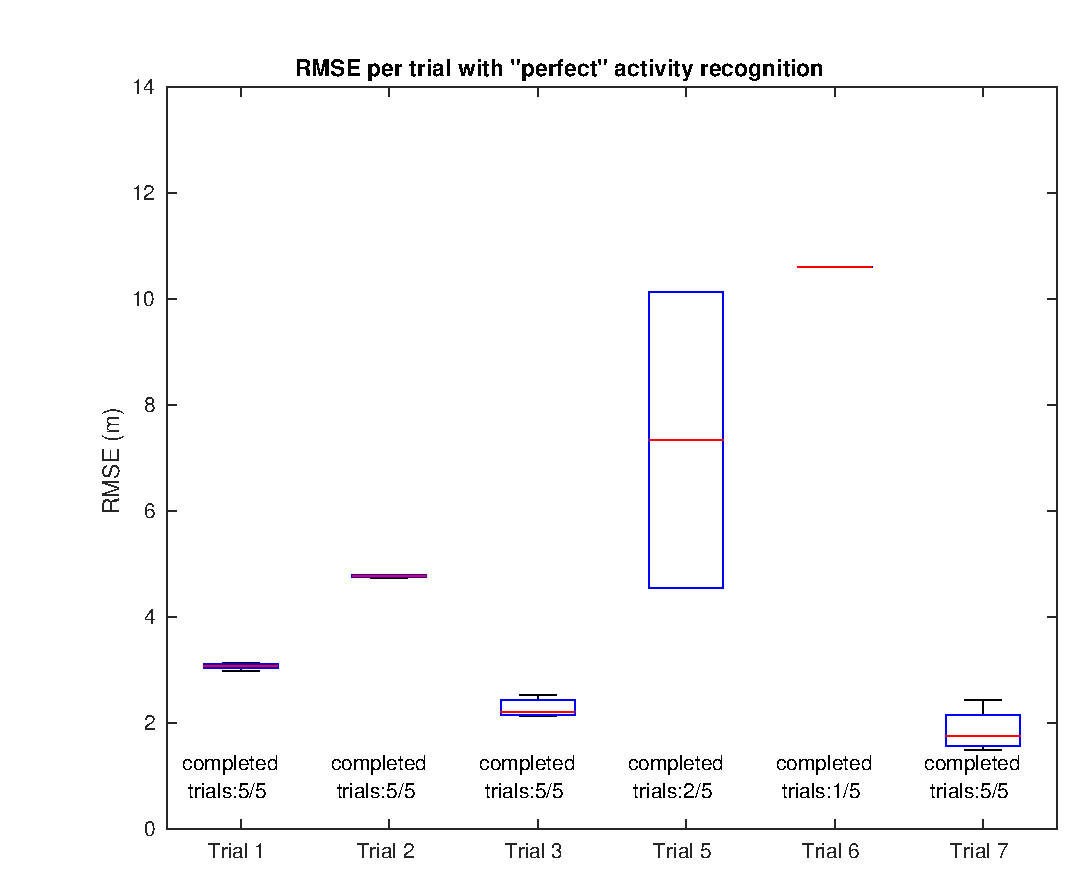
\includegraphics[width=0.6\textwidth]{images/20201116_1332_RMSE_per_trial_with_perfect_activity_recognition}
	\caption[Particle Filter position estimation performance with door interaction]{Particle Filter position estimation performance with rough video generated estimate using manually indicated door interactions}	
	\label{fig:pf_boxplot}
\end{figure}

The results show that for trials 1 to 3 and trial 7 that all five itterations were completed, with their individual itterations have similar RMSE values. The RMSE per trial do vary, which can be explained by looking at the trajectory that the system generates, which will be done in the discussion.\par 

\subsubsection{Without activity}
The same SHS trajectory were used, however now door interaction landmarks were not used as measurement update. The results can be found in \cref{fig:pf_boxplot_no_doors}.

\begin{figure}[H]
	\centering
	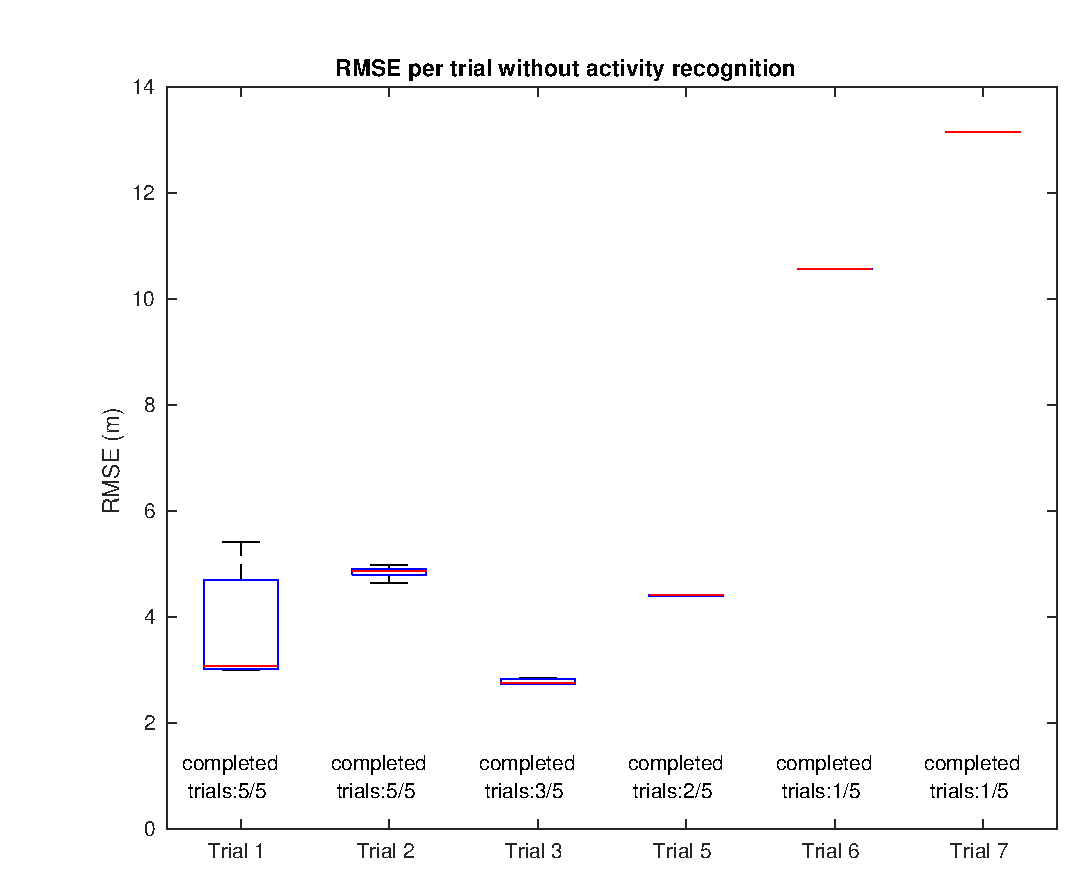
\includegraphics[width=0.7\textwidth]{images/20201116_1333_RMSE_per_trial_without_activity_recognition}
	\caption[Particle Filter position estimation performance without door interaction]{Particle Filter position estimation performance without door interaction measurment update, 5 itterations per trial. Number under "completed" indicates how many trials had particles surviving for the whole SHS trajectory.}
	\label{fig:pf_boxplot_no_doors}
\end{figure}

\textcolor{purple}{
	things to notice
	\begin{itemize}
		\item Trial one has very different RMSE value per run
		\item Strangely it did not have much effect on lopen1.2
		\item Although the RMSE of lopen1.3 is similar to the one with door activity two of the 5 trials did not complete the SHS track. This means that all particles.
		\item So far this does indicate that having activity recognition does help with position estimation within a particle filter
\end{itemize}}

